\documentclass[10pt,compress,usetitleprogressbar,mathserif]{beamer}
\usepackage[spanish, es-tabla,es-noquoting,es-noshorthands]{babel}
\usepackage{etex}
\usepackage{tikz} % Tikz (para el tema)
\usepackage{showexpl} % ???
\usepackage{amsthm}  %%
\usepackage{amsmath} % Matemáticas
\usepackage{amssymb} %%
\usepackage{graphicx} % Imágenes
\usepackage{adjustbox} % Tamaño de tablas
\graphicspath{{img/}} % Ruta de las imágenes
\usepackage{pgfplotstable} %Tablas
\usepackage{booktabs}% http://ctan.org/pkg/booktabs

\pgfplotstableset{ % Estilo de todas las tablas
sci zerofill,
column type/.add={|}{},
every last column/.style={column type/.add={}{|}},
every head row/.style={before row=\hline},
after row=\hline,
% tex.stackexchange.com/questions/110233
row predicate/.code={%
\pgfmathparse{int(mod(#1,5))}
\ifnum\pgfmathresult=0\relax
\else\pgfplotstableuserowfalse\fi}
}

\usepackage{listings} % Códigos

\definecolor{backg}{HTML}{F2F2F2}    % Fondo
\definecolor{comments}{HTML}{BDBDBD} % Comentarios
\definecolor{keywords}{HTML}{08388c} % Palabras clave
\definecolor{strings}{HTML}{0489B1}  % Strings

\lstset{
language=C++,
basicstyle=\ttfamily\small,
breaklines=true,
backgroundcolor=\color{backg},
keywordstyle=\color{keywords},
commentstyle=\color{comments},
stringstyle=\color{strings},
tabsize=2,
% Acentos, ñ, ¿, ¡ (tex.stackexchange.com/questions/24528)
extendedchars=true,
literate={á}{{\'a}}1 {é}{{\'e}}1 {í}{{\'i}}1 {ó}{{\'o}}1
         {ú}{{\'u}}1 {ñ}{{\~n}}1 {¡}{{\textexclamdown}}1
         {¿}{{?`}}1 {->}{{$\rightarrow$}}1 {=>}{{$\Rightarrow$}}1
}

% Solarized palette
\definecolor{solarizedBase03}{HTML}{002B36}
\definecolor{solarizedBase02}{HTML}{073642}
\definecolor{solarizedBase01}{HTML}{586e75}
\definecolor{solarizedBase00}{HTML}{657b83}
\definecolor{solarizedBase0}{HTML}{839496}
\definecolor{solarizedBase1}{HTML}{93a1a1}
\definecolor{solarizedBase2}{HTML}{EEE8D5}
\definecolor{solarizedBase3}{HTML}{FDF6E3}
\definecolor{solarizedYellow}{HTML}{B58900}
\definecolor{solarizedOrange}{HTML}{CB4B16}
\definecolor{solarizedRed}{HTML}{DC322F}
\definecolor{solarizedMagenta}{HTML}{D33682}
\definecolor{solarizedViolet}{HTML}{6C71C4}
\definecolor{solarizedBlue}{HTML}{268BD2}
\definecolor{solarizedCyan}{HTML}{2AA198}
\definecolor{solarizedGreen}{HTML}{859900}

\usetheme{epstfg}
\setbeamertemplate{note page}[compress]
\setbeamertemplate{itemize subitem}{\tiny\raise1.5pt\hbox{\donotcoloroutermaths$\blacktriangleright$}}
\title{Práctica 4}
\author{Pablo Baeyens \and Antonio Checa \and Iñaki Madinabeitia \and José Manuel Muñoz \and Darío Sierra}
\date{Algorítmica}
\def\inline{\lstinline[basicstyle=\ttfamily]}

\begin{document}
\maketitle

\begin{frame}{Índice}
  \tableofcontents
\end{frame}
\section{Estación de ITV}

\begin{frame}{Problema}
\begin{itemize}
	\item Una estación de ITV tiene $m$ líneas.
	\pause
	\item Hay $n$ vehículos que quieren repartirse entre las líneas. El vehículo $i$
	requiere un tiempo $T_i$ para ser inspeccionado.
	\pause
	\item Se pretende repartir los vehículos en las líneas de forma que la última
	inspección termine lo antes posible.
\end{itemize}
\pause

Presentaremos algoritmos con el formato:
\begin{description}
 \item[Entrada:] Vector de tiempos de los coches $T$ y número de líneas $m$
 \item[Salida:] Vector que indica en la posición $i$ a qué línea va el coche $i$-ésimo
\end{description}
\end{frame}

% TODO: descripción del greedy

% TODO: descripción del backtrack

\begin{frame}{Eficiencia}
	\begin{itemize}
		\item Problema: \textbf{Tamaño del árbol}
		\pause
		\item El tiempo crece al aumentar las \textbf{líneas} y/o los \textbf{coches}
		\pause
		\item ¿Solución para estudiar la eficiencia?
		\pause
		\item \textbf{Fijamos} el número de filas y dejamos variable el número de coches
	\end{itemize}
\end{frame}

\begin{frame}{Eficiencia-Tiempo de ejecución}
	\begin{center}
		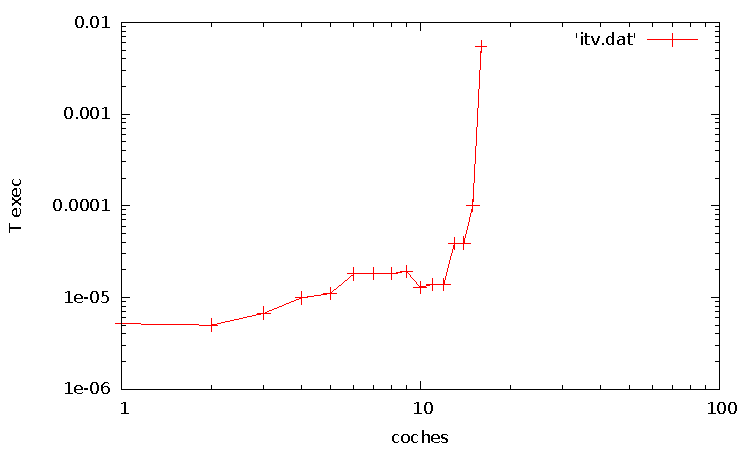
\includegraphics[width = \linewidth]{img/itvEficiencia}
	\end{center}
\end{frame}

\begin{frame}{Eficiencia-Comparación con Greedy}
	\begin{itemize}
		\item Vamos a analizar qué hemos ganado y qué perdido.
		\pause
		\item Está claro que los resultados son mejores, pero, ¿Y el tiempo?
		\pause
		\item Para $5$ líneas y $18$ coches el greedy tarda varios órdenes de magnitud menos.
		\item \textbf{¿Cuánto hemos ganado exactamente?}
		

	\end{itemize}
	\begin{center}
			\begin{tabular}{c|c|c}
				Coches	& Greedy  & Backtracking  \\ 
				17	& 190.33 &  209.09\\ 
				18	& 209.09 & 200.59
			\end{tabular}
			
	\end{center}

\end{frame}

\begin{frame}{Eficiencia-Gráfica Greedy vs Backtracking}
	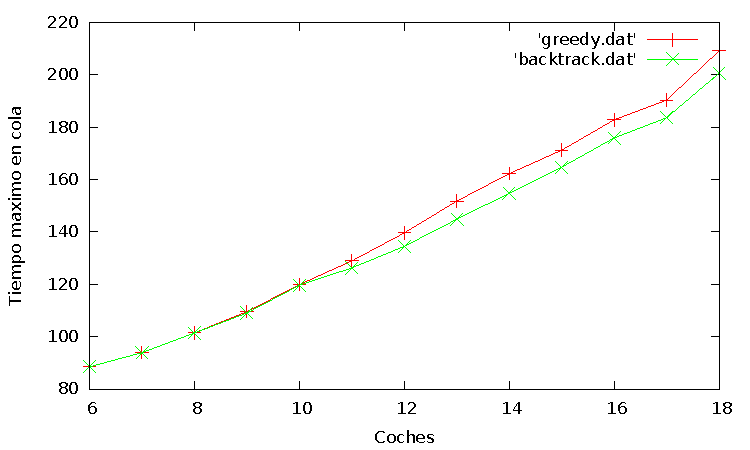
\includegraphics[width = \linewidth]{./img/comp.pdf}
\end{frame}


\section{El problema del viajante de comercio}

\begin{frame}{Problema}
Hallar el recorrido con distancia mínima en un conjunto de
ciudades que pase por todas las ciudades y regrese al punto inicial.

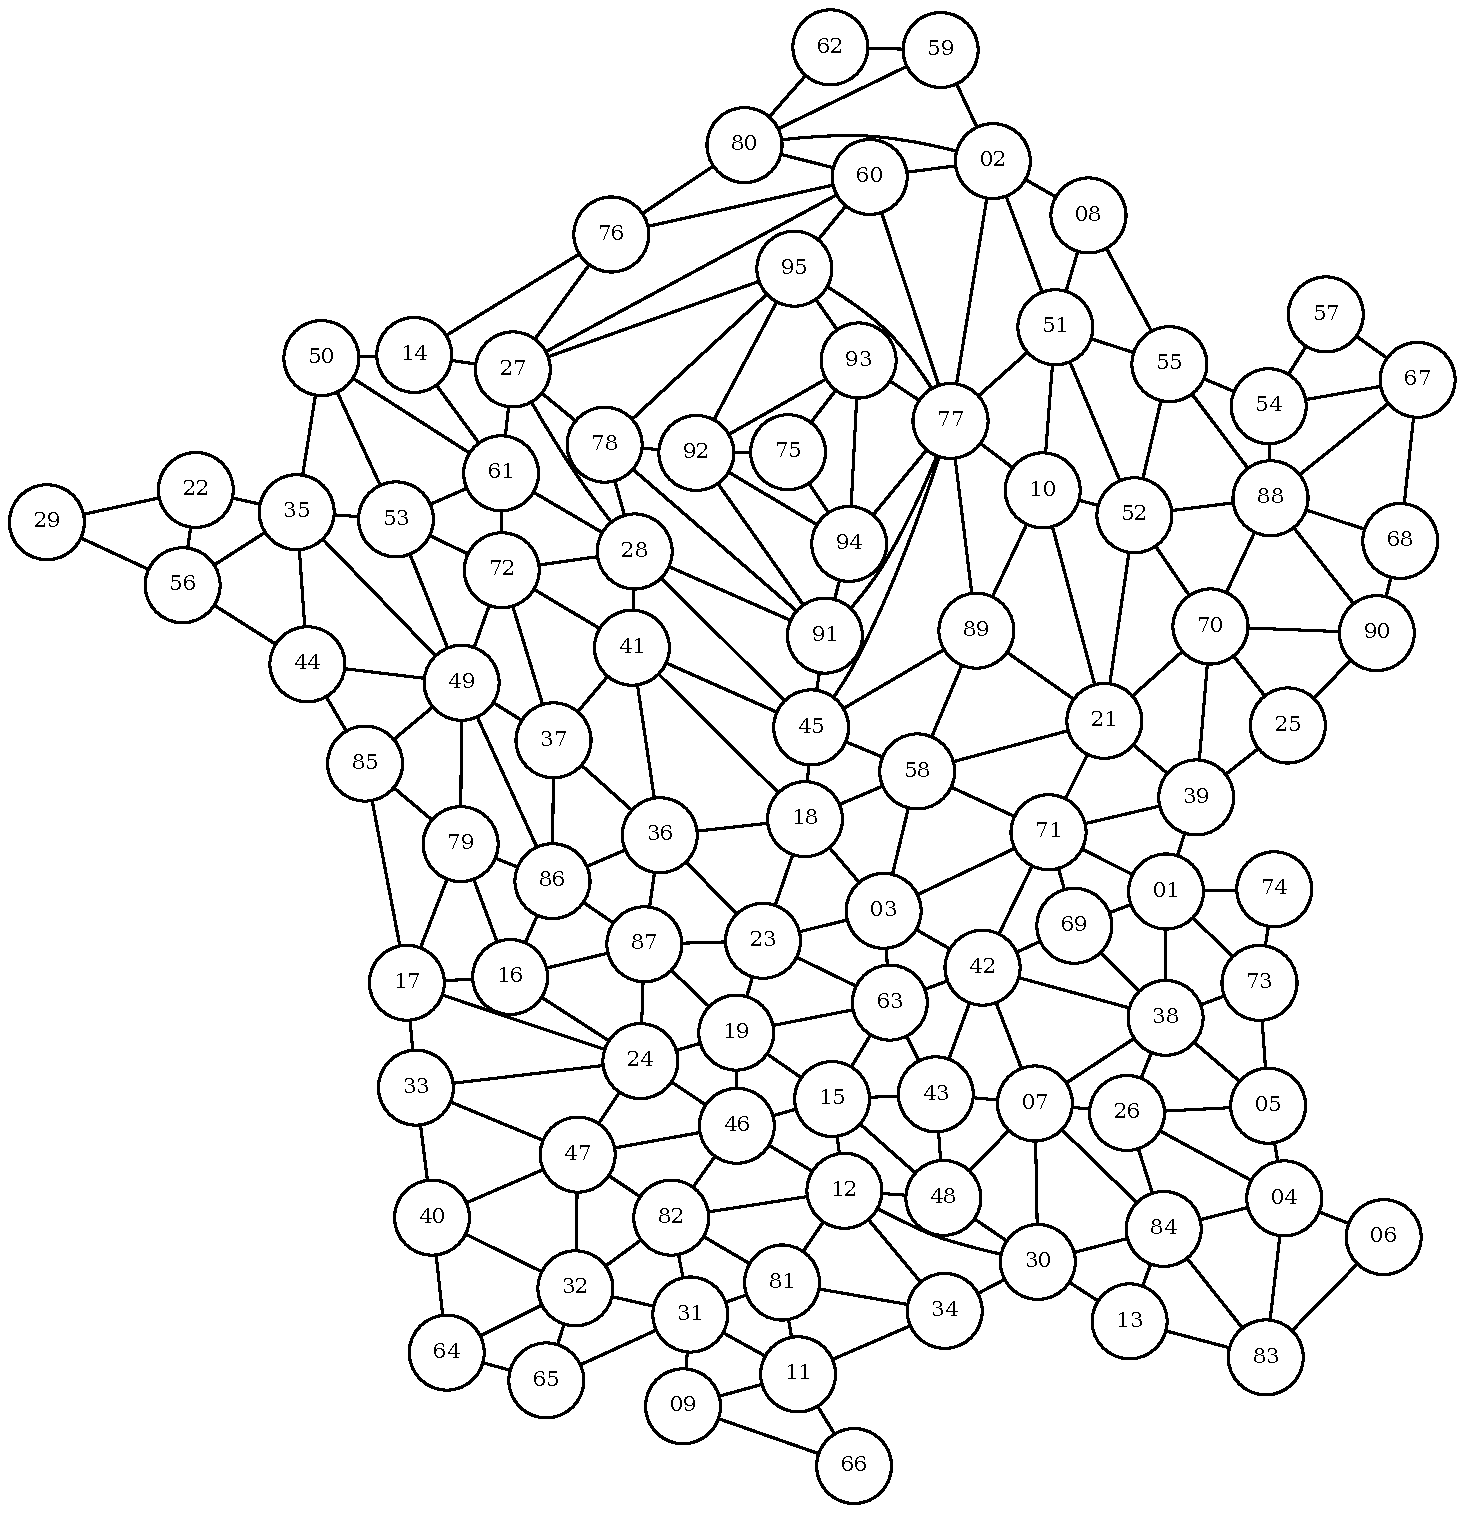
\includegraphics[width=.5\textwidth]{img/Francia} \centering
\end{frame}

\begin{frame}{Algoritmos}
\begin{description}
 \item[Entrada:] Ficheros con ciudades indicadas como puntos en el plano según sus
 coordenadas.
 \item[Salida:] \texttt{vector<int>} con el orden en el que se recorren las ciudades.
\end{description}
\end{frame}

% TODO: todo lo posterior

\begin{frame}{\texttt{Grafo}}
Un grafo consta de:

\begin{itemize}
  \item Una \textbf{cantidad de nodos}: \texttt{nodos}.
  \item Una \textbf{matriz de pesos}: \texttt{lados}.
\end{itemize}
\end{frame}

\subsection{Ramificación y acotación}

\begin{frame}{Algoritmo general}
  Iniciamos:
  \begin{itemize}
    \item La cola con la solución parcial \texttt{[0]}
    \item La mejor solución con un algoritmo \textit{greedy} (vecino más cercano)
  \end{itemize}
\end{frame}

\begin{frame}{Algoritmo general}
  Mientras la cola no esté vacía, coge el primer elemento:
  \begin{itemize}
    \item Si \textbf{puede formarse una solución completa}, comprueba si es mejor que la mejor encontrada. En tal caso actualizala y borra los nodos con peor cota.
    \item En \textbf{otro caso}, para cada ciudad no visitada forma una nueva solución parcial. Añádela a la cola si su cota es mejor que la mejor solución.
  \end{itemize}
\end{frame}

\subsubsection{Cotas}

\begin{frame}{Cota del mínimo}
  Calcular la longitud del recorrido inicial y suma la menor distancia de cada ciudad no incluida en la solución parcial con sus relacionadas.
\end{frame}

\begin{frame}{Arbol generador}
  Calcular la longitud del recorrido que se lleva hasta ese momento, y suma la longitud del árbol generador minimal de los nodos que faltan junto al último nodo del camino. Además, se suma la mínima longitud del primer nodo a otro más.

  %% Aquí pintad en pizarra que si no, no lo entiende ni dios, y es una tontería
\end{frame}

\subsection{Vuelta atrás}

\begin{frame}{Backtracking}
  Desde un nodo inicial, vamos tomando todas las posibilidades mediante una llamada recursiva. Si al añadir un nodo hace que el camino mida más que nuestra mejor longitud hasta el momento, se deja esa posibilidad, y se vuelve atrás.
\end{frame}

\begin{frame}[fragile]{Llamada inicial backtracking}
\begin{lstlisting}
vector<int> tsp_backtracking(const Grafo<peso_t>& g) {
	vector<int> primera_solucion = tsp_greedy(g);
	int mejor_longitud = longitud(primera_solucion,g);
	vector<int> inicial = {0};
	vector<int> solucion; // Se modifica

	tsp_back_rec(solucion,inicial,mejor_longitud,g);

	return solucion;
}
\end{lstlisting}
\end{frame}

\subsection{Comparativa de los algoritmos}

\begin{frame}{5 ciudades (tiempos)}
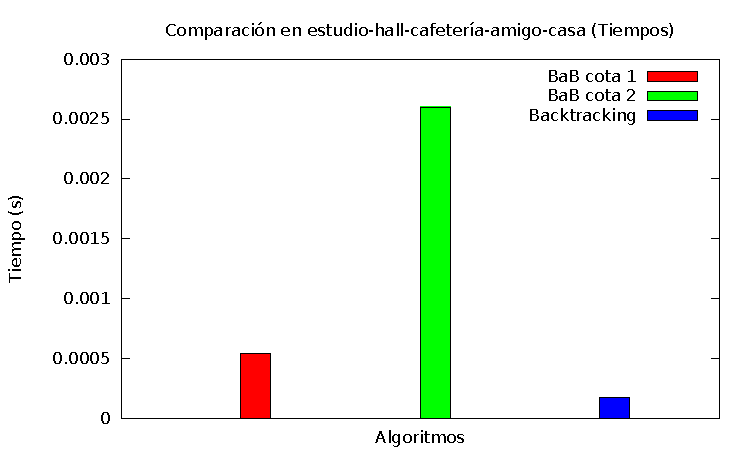
\includegraphics[width=\textwidth]{img/barras_e-h-c-a-c5_t}
\end{frame}

\begin{frame}{5 ciudades (nodos expandidos)}
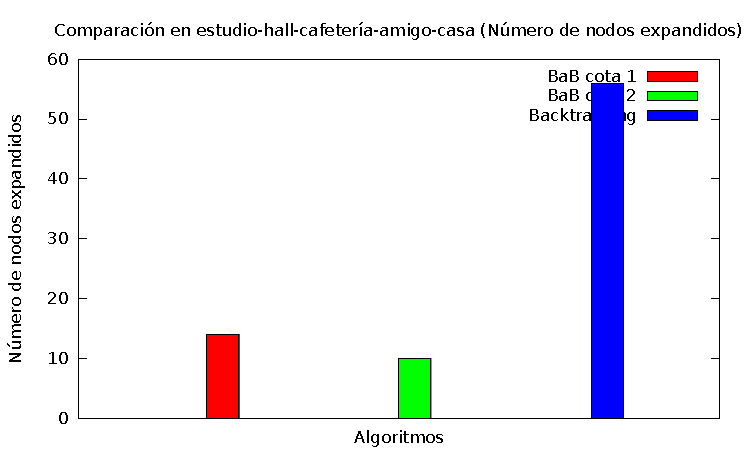
\includegraphics[width=\textwidth]{img/barras_e-h-c-a-c5_nodos}
\end{frame}

\begin{frame}{5 ciudades (Podas)}
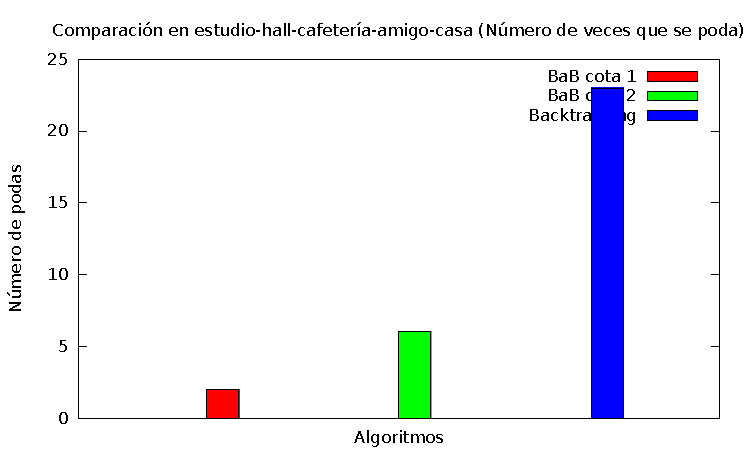
\includegraphics[width=\textwidth]{img/barras_e-h-c-a-c5_poda}
\end{frame}

\begin{frame}{5 ciudades (Cola)}
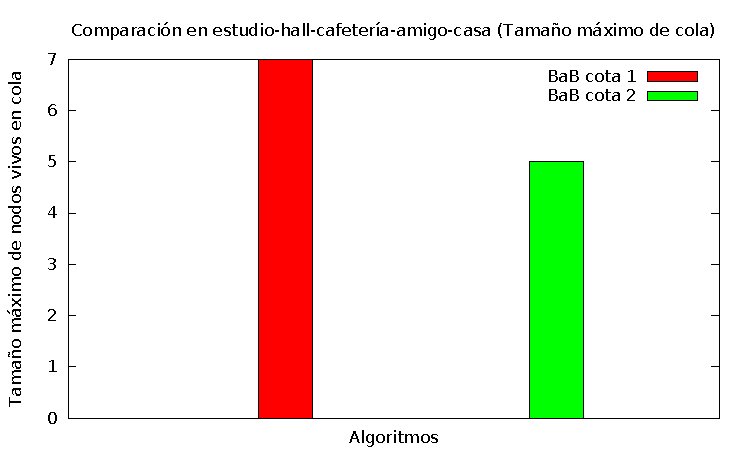
\includegraphics[width=\textwidth]{img/barras_e-h-c-a-c5_cola}
\end{frame}

\begin{frame}{10 ciudades (tiempos)}
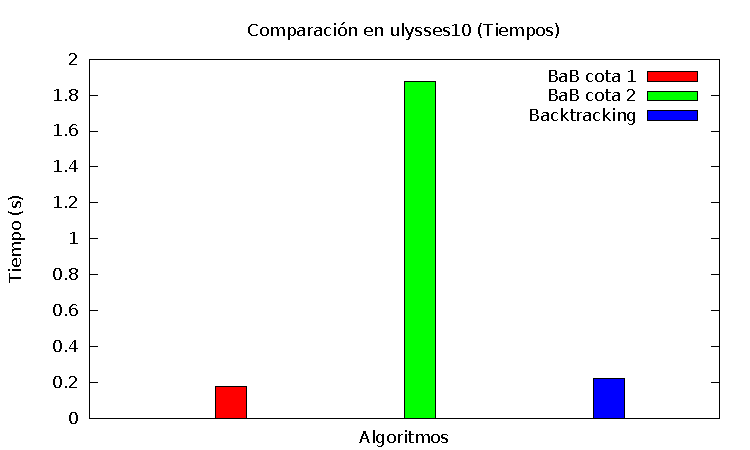
\includegraphics[width=\textwidth]{img/barras_ulysses10_t}
\end{frame}

\begin{frame}{10 ciudades (nodos expandidos)}
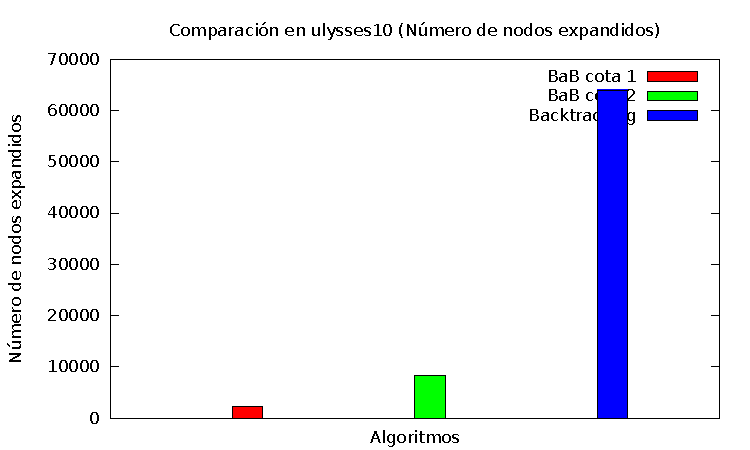
\includegraphics[width=\textwidth]{img/barras_ulysses10_nodos}
\end{frame}

\begin{frame}{10 ciudades (Podas)}
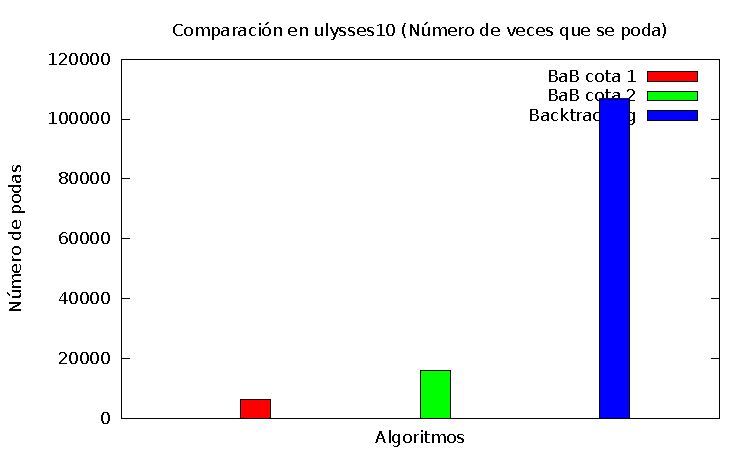
\includegraphics[width=\textwidth]{img/barras_ulysses10_poda}
\end{frame}

\begin{frame}{10 ciudades (Cola)}
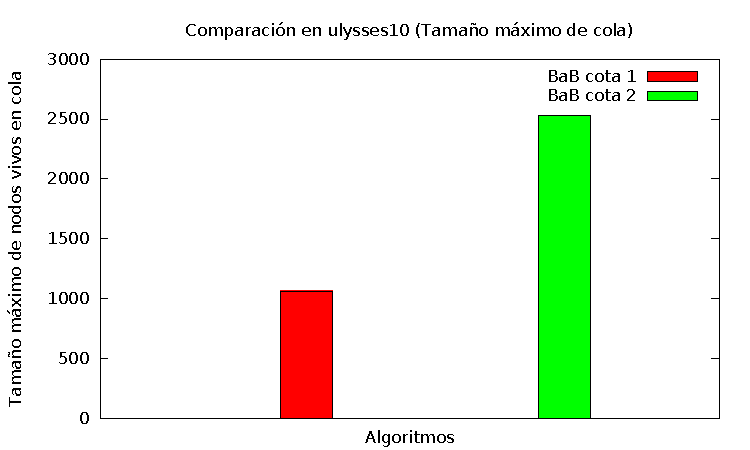
\includegraphics[width=\textwidth]{img/barras_ulysses10_cola}
\end{frame}

\begin{frame}{12 ciudades (tiempos)}
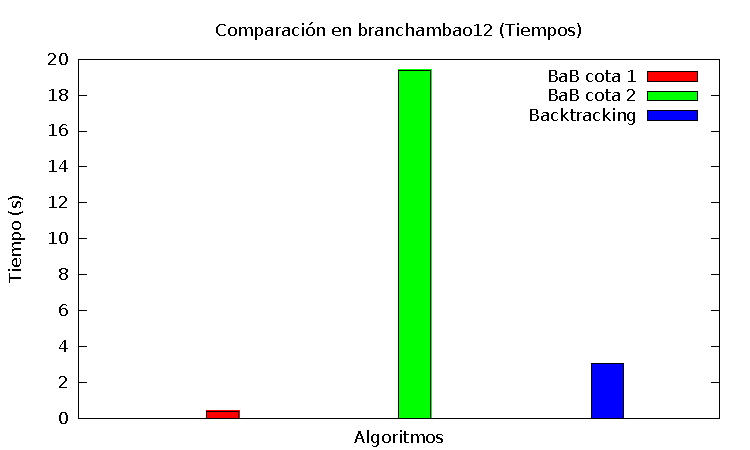
\includegraphics[width=\textwidth]{img/barras_branchambao12_t}
\end{frame}

\begin{frame}{12 ciudades (nodos expandidos)}
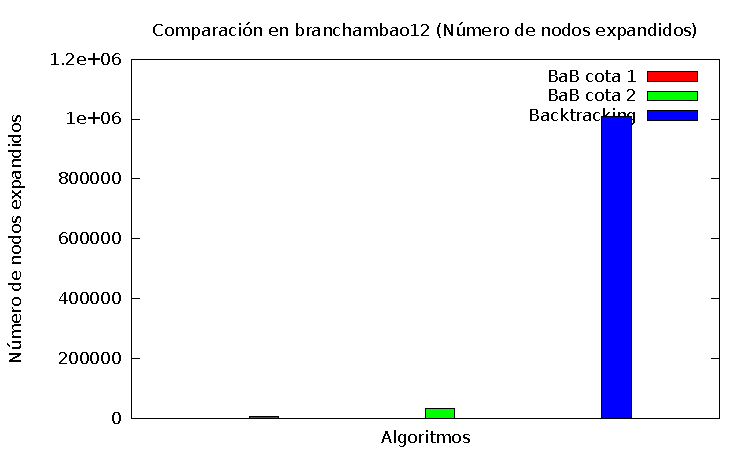
\includegraphics[width=\textwidth]{img/barras_branchambao12_nodos}
\end{frame}

\begin{frame}{12 ciudades (Podas)}
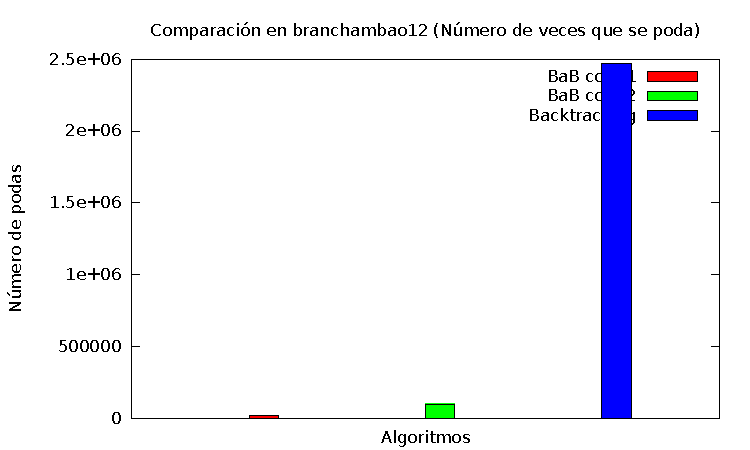
\includegraphics[width=\textwidth]{img/barras_branchambao12_poda}
\end{frame}

\begin{frame}{12 ciudades (Cola)}
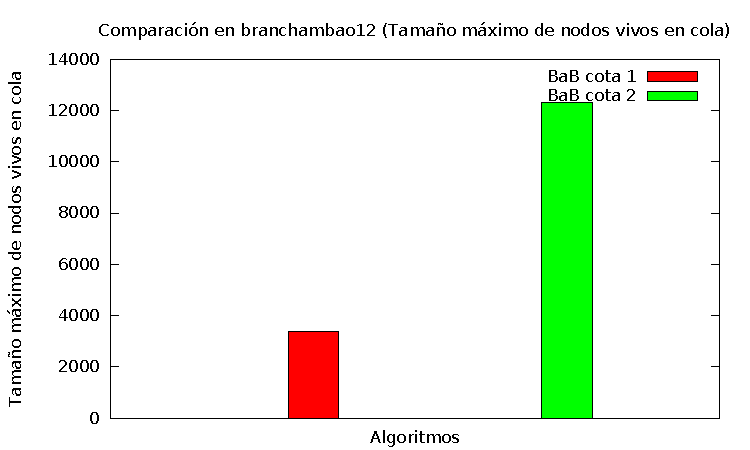
\includegraphics[width=\textwidth]{img/barras_branchambao12_cola}
\end{frame}

\end{document}
